% !TEX root = ../Thesis.tex
% !TEX output_directory
\documentclass[11pt,a4paper,english,greek,twoside]{../Thesis}

\begin{document}
\chapter{Ανασκόπηση των BCIs που κάνουν χρήση ΗΕΓ} \label{chap:survey}

\section{State of the Art χρήσεις και κατευθύνσεις}

\subsection{Τι ορίζουμε ως State of the Art BCI}

\par Γενικά η σύγκριση μεταξύ BCI, στην πλειοψηφία των περιπτώσεων δεν είναι δυνατή. Αυτές οι διεπαφές είναι τόσο πολυμεταβλητά συστήματα, όπου είναι σχεδόν αδύνατον να αναπαραχθούν τα ίδια αποτελέσματα δεύτερη φορά, ακόμα και αν διατηρηθούν οι συνθήκες του πειράματος όσο το δυνατόν αναλλοίωτες. Συνεπώς έχοντας ως μοναδικό κριτήριο, μόνο τις επιδόσεις που αναφέρονται σε κάθε δημοσίευση, δεν μπορούμε με ασφάλεια να κάνουμε συγκρίσεις. 

\par  Μέχρι το 2000 οι υψηλότερες επιδόσεις ITR που είχαν επιτευχθεί στα BCI, κυμαίνονταν μεταξύ 5–25bits/min, \cite{wolpaw2000brain}, ενώ σήμερα αγγίζουν τα 350bits/min. Ωστόσο, αν παρατηρήσουμε την ακρίβεια που πετυχαίνει ένα τέτοιο high speed BCI, σπάνια θα ξεπερνάει το 90\%, επίδοση που πολλά από τα σύγχρονα και παλαιότερα "αργά" BCIs, υπερβαίνουν με ευκολία. Εδώ φαίνονται και οι δύο διαφορετικές προσεγγίσεις που κυριαρχούν σε αυτόν τον ερευνητικό τομέα, η μεγιστοποίηση του ITR με κάθε κόστος, και από την αντίπερα όχθη, η μεγιστοποίηση της ακρίβειας, ακόμα και αν το σύστημα είναι πιο αργό. Τα στατιστικά δείχνουν πως οι χρήστες προτιμούν BCIs με μικρότερο ITR αλλά μεγαλύτερη ακρίβεια, καθώς γίνονται πολύ λιγότερα λάθη. Επίσης, συνήθως τα BCI με πολύ υψηλές επιδόσεις όσον αφορά το ITR χρησιμοποιούν δεκάδες ΕΟΔ, πράγμα το οποίο προκαλεί κούραση στον χρήστη. Συνήθως οι ερευνητικές ομάδες που ανήκουν περισσότερο στον ιατρικό τομέα, στοχεύουν στην μεγιστοποίηση της ακρίβειας και της άνεσης του χρήστη, ενώ αυτές που ανήκουν στον πιο τεχνικό τομέα στοχεύουν στην μεγιστοποίηση του ITR. 

\par Γι αυτό το λόγο, η αναζήτηση των state of the art εργασιων, έγινε με κριτήριο την ταχύτητα του σύστήματος (ITR), την ακρίβεια και την άνεση που νιώθει ο χρήστης, καθώς και την εφαρμογή πρωτοπόριακών μεθόδων, ακόμα και αν δεν επιτεύχθηκαν υψηλές επιδόσεις.

\par Ένα διάγραμμα με τις καλύτερες επιδόσεις όσον αφορά τον ITR, μέχρι το 2015, φαίνεται στην εικόνα \ref{fig:survey} όπου φαίνεται και η μέγιστη επίδοση μέχρι τότε, αγγίζοντας τα 320bits/min (5.33bits/s) \cite{Chen2015-oh}. Η ίδια ερευνητική ομάδα, το 2018 \cite{Nakanishi2018-sc}, αναζητώντας βελτιώσεις στο προηγούμενο σύστημα τους, πέτυχαν ακρίβεια 89.83±6.07\% kai ITR ίσο με 325.33±38.17 bits/min για σύγχρονη (synchronous, cue-based) online διεπαφή, επίδοση που αποτελεί την υψηλότερη αναφερθείσα στην βιβλιογραφία. Ωστόσο αναφέρουν πως στην ασύγχρονη εκδοχή του συστήματός τους, η μέση επίδοση των χρηστών έπεσε στα 198.67±50.48 bits/min. Η διεπαφή που ανέπτυξαν είναι ένας speller όπου τα γράμματα και οι αριθμοί είναι διατεταγμένα σε έναν πίνακα 8x5, και καθένα από τα 40 κελιά, είναι μια ΕΟΔ διαφορετικής συχνότητας. Ωστόσο μια σημαντική διαφορά με άλλες εργασίες είναι πως κάθε ΕΟΔ ταλαντώνεται με διαφορετική φάση, η οποία με την σειρά της λαμβάνεται υπόψιν κατά την επεξεργασία των σημάτων. 

\begin{figure}[H]
    \centering     %%% not \center
    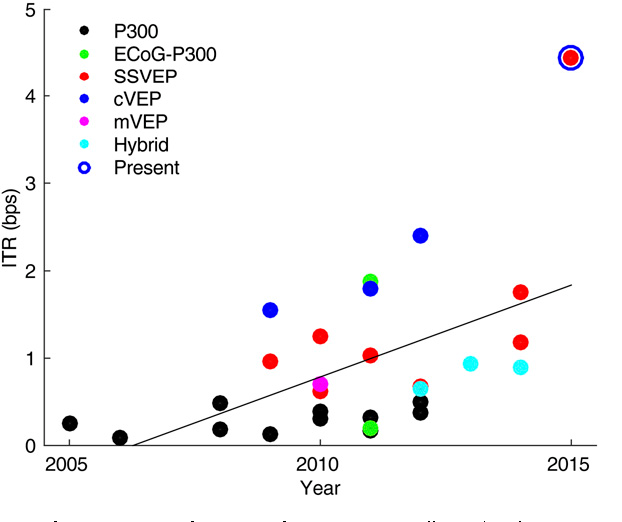
\includegraphics[scale=0.4]{{{ImagesSSVEP/survey}.png}}
    \caption{ Το διάγραμμα λειτουργί
    }
    \label{fig:survey}
\end{figure}

\par 


\section{Παρόμοιες εργασίες - Διεπαφές βασισμένες σε Emotiv Epoc και SSVEPs}

\par Σε αυτό το σημείο θα κάνουμε μια σύντομη παρουσίαση στις πιο cited (\textbf{πως το λεμε στα ελληνικα}) δημοσιεύσεις που βρήκαμε στη βιβλιογραφία, χρησιμοποιώντας ως λέξεις κλειδιά τις "Emotiv", "Epoc", "SSVEP". Ο σκοπός είναι ενημερωθούμε για τις επιδόσεις διεπαφών που χρησιμοποίησαν παρόμοιο υλικό με εμάς, και να αποτελέσουν ένα σημείο αναφοράς και σύγκρισης των δικών μας αποτελεσμάτων.

\par Η πιο cited έρευνα πάνω στο θέμα Epoc - SSVEP, δημοσιεύτηκε το 2012 \cite{Liu2012-qj} και ο σκοπός ήταν η σύγκριση του Epoc με ένα σύστημα ιατρικών προδιαγραφών, το  g.USBamp. H μέθοδος που χρησιμοποίησαν ήταν η CCA, πραγματοποίησαν offline και online ανάλυση σε τέσσερις χρήστες. Στην οffline χρησιμοποιήθηκαν 16 ΕΟΔ και χρονικά παράθυρα 6sec, ενώ στην online 6 ΕΟΔ. Τα αποτελέσματα της offline ανάλυσης για το EPOC ήταν 82.99±4.98\% ακρίβεια με ITR 28.06±6.45 bits/min. Στο online σκέλος, οι επιδόσεις είναι 95.83±3.59\%, με ITR 18.99±1.68 bits/min και χρόνο αναγνώρισης για κάθε εντολή 5.25±2.14 sec. Ωστόσο δεν διασαφηνίζουν αν αυτά τα αποτελέσματα αφορούν το Epoc, η τον g.USBamp, καθώς και δεν αναφέρουν αν η online διεπαφή ήταν σύγχρονη, έτσι ώστε να μπορούν να υπολογίσουν τον ITR. 

\par Σε μια άλλη δημοσίευση \cite{noauthor_undated-vk}, πάλι ο Epoc συγκρίθηκε με έναν ακριβότερο εγκεφαλογράφο, αλλά σε τελείως διαφορετικές καταστάσεις από την προηγούμενη εργασία. Ο σκοπός ήταν ο έλεγχος ενός παιχνιδιού, κάνοντας χρήση μόνο μιας ΕΟΔ, και χρησιμοποιώντας ως μέθοδο ανίχνευσης SSVEP, κατάτμηση του σήματος στο πεδίο του χρόνου και averaging \cite{Friman2007-xm}. Παρότι το πλαίσιο εφαρμογής αυτής της δημοσίευσης διαφέρει σημαντικά από την παρούσα εργασία, είναι σημαντικό να αναφερθεί το γεγονός πως αυτή η διεπαφή δεν έμεινε μόνο στο εργαστήριο, αλλά δοκιμάστηκε από 25 άτομα, σε εξωτερικό χώρο, όπου 9 από αυτά την χειρίστηκαν με άνεση.

% Φαίνεται πως το Epoc αποδίδει καλά στα σήματα P300 αν και δεν έχει ηλεκτρόδια εκει που πρεπει Debener S, Minow F, Emkes R, Gandras K, de Vos M: How about taking a low-cost, small, and wireless EEG for a walk?. Psychophysiology. 2012, 49: 1617-1621.
% [[
% [HTML] Performance of the Emotiv Epoc headset for P300-based applications
% M Duvinage, T

%D. Matthieu, C. Thierry, P. Mathieu, A P300-based quantitative comparison between the Emotiv EPOC headset and a medical EEG device. Int. J. Biomed. Eng. 12(56), 201 (2013)

\par Μια άλλη πολύ σημαντική έρευνα, έγινε το 2014 στο πανεπιστήμιο UCSD \cite{Lin2014-cp}, και ανοίγει τον δρόμο για την χρήση των BCI εκτός εργαστηρίου, σε κανονικές συνθήκες. Συγκεκριμένα, κάνοντας χρήση του Epoc, δοκιμάστηκε το κατά πόσο είναι δυνατή η υλοποίηση μια SSVEP διεπαφής, την ώρα που ο χρήστης περπατάει με διάφορες ταχύτητες. Στα αποτελέσματά τους παρουσίασαν πως για ταχύτητες έως και 0.89m/s, μπορεί να επιτευχθεί ITR έως και 12bits/min. Επιπλέον, παρουσιάζονται και οι επιδόσεις για την περίπτωση όπου ο χρήστης είναι ακίνητος, μέση ακρίβεια 76.60 ± 21.74\% με ITR: 14.38 ± 9.04 για 17 χρήστες.
Το γεγονός σε αυτή την δημοσίευση χρησιμοποιήθηκαν τέσσερις ΕΟΔ με συχνότητες 9,10,11 και 12 Hz, και φυσικά ο Epoc, την καθιστούν αρκετά παρόμοια με την παρούσα διπλωματική, και συνεπώς θα έχει αξία να δούμε αν τα αποτελέσματα μας θα είναι συγκρίσιμα.
% στο ιδιο πεηπερ λεει :The amplitude of SSVEP has been found to be largely modulated by visual spatial attention [28]. As a consequence, the loss of focus could reduce visual attention and thereby lead to the decreased SSVEP amplitude.
% Επισης εδω καταληγουν πως ο Εποκ εχει διαφορα προβληματακια, και δεν πρεπει να χρησιμοποιείται σε σοβαρες εφαρμογες (να το βαλω στο τελος στα συμπερασματα)

\begin{figure}[H]
    \centering     %%% not \center
    \subfigure[]{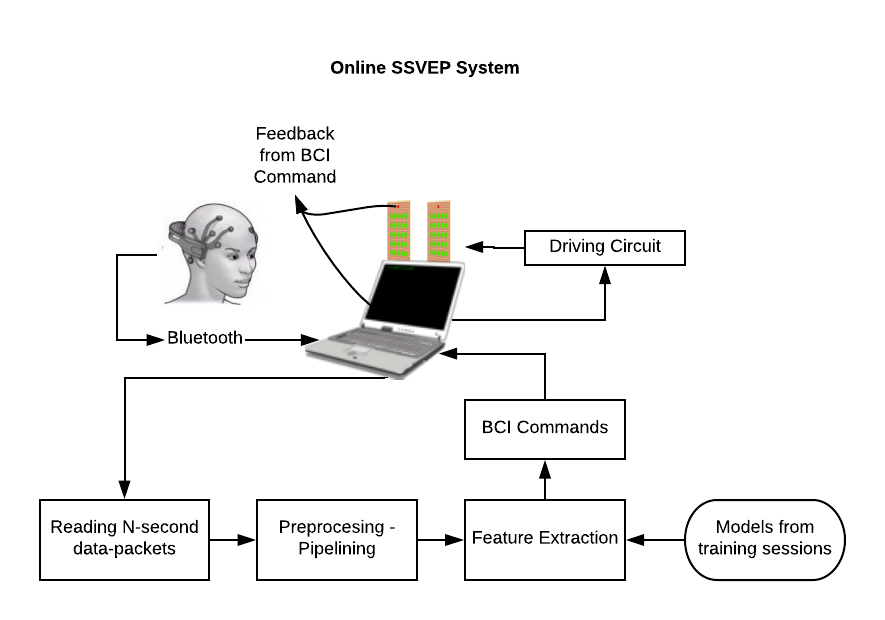
\includegraphics[scale=0.5]{{{ImagesSSVEP/online}.png}}}
    \subfigure[]{
\includegraphics[scale=0.3]{{{ImagesSSVEP/task_game}.png}}}
    \caption{a) Το γενικό διάγραμμα λειτουργίας της οnline BCI διεπαφής, b) το απλό παιχνίδι λαβυρίνθου στο οποίο ο χρήστης έπρεπε να κατευθύνει το avatar του (pacman) πρoς το πράσινο άστρο. }
    \label{fig:driver_circuit}
\end{figure}

\par Η μόνη εργασία που βρήκαμε, η οποία να χρησιμοποιεί ΕΟΔ με υψηλές συχνότητες 28, 30, 32 και 34 Hz, είναι η \cite{Holewa2014-an}, και τα αποτελέσματα 73.75\% ακρίβεια, με ITR 11.36, αν και υπολείπονται με τα προηγούμενα, είναι πολύ ικανοποιητικά δεδομένου του χαμηλού SNR που παρουσιάζουν τα SSVEP στις συχνότητες αυτές. \textbf{δεν μου το ανοιγει το scihub για να δω λεπτομερειες}
% παλι δν περιγραφουν τπτ απο την μεθοδο τους. 


%http://www.koreascience.or.kr/article/ArticleFullRecord.jsp?cn=PJJNBT_2015_v25n3_254
εδω πετυχαινουν 70\% με LDA kai SVM

\par Τέλος, να αναφερθούμε και σε μια δημοσίευση που ισχυρίζεται πως το Epoc δεν είναι κατάλληλο για την ανίχνευση SSVEPs \cite{noauthor_undated-hj}. Ο αρχικός σκοπός της εργασίας ήταν η χρήση νευρωνικού δικτύου για την κατηγοριοποίηση εγκεφαλικών σημάτων που παράγει ο χρήστης από μόνος του, χωρίς την επίδραση εξωτερικών διεγέρσεων (active BCI). Ωστόσο, αναζητώντας διαφορετικούς τρόπους υλοποίησης, στράφηκαν προς τα SSVEPs, δοκιμάζοντας να ανιχνεύσουν τα δυναμικά χρησιμοποιώντας μια ΕΟΔ συχνότητας 7Hz.

Controlling mobile Spykee robot using Emotiv neuro headset 2013 china
cited by 19
Edw οι τυπαδες πανε να εξαγουν 4 εντολες με mental controls, οχι με προκλητα δυναμικα δλδ, και στην συνεχεια αναρρωτιουνται πως αλλιως μπορουνε. προτεινουν SSVEP, αλλα καταλήγουν πως to emotiv dn anixneyei ssvep (οτι να ναι), επειδη τα Ο1 και Ο2 δεν ειναι καταλληλα για αυτη τη δουλεια (οτι να ναι παλι)


\end{document}